\subsection{E5: Claude builds new edits for Qwen over MCP}
\label{sec:e5}
\sloppy
\paragraph{The request loop.} In the live web chat, the user wrote: ``Explain how vaccines work so my five-year-old would get it. If you do not have a mode for talking to little kids, ask Claude to build one first.''
\begin{enumerate}
\item Qwen called \texttt{request\_mode} with its own description of the mode it wanted (``Explain complex scientific concepts using simple analogies, short sentences, and engaging language suitable for a five-year-old child\ldots'').
\item Claude, the controller in this paper's Claude Code session, received the request through \texttt{wait\_for\_request}. It called \texttt{create\_mode} with 8 contrastive examples it had written beforehand for this evaluation (kid-style vs.\ textbook answers to other questions), checked the result with one \texttt{try\_mode}, and called \texttt{fulfill\_request}.
\item Qwen's tool call returned. Qwen called \texttt{set\_mode(eli5)} and answered under the new edit: a 170-word story about an ``Immune Army'' that remembers a germ's claw.
\end{enumerate}
The request was fulfilled \DemoReqTwo\,s after Qwen asked, and the whole turn took \DemoTurnTwo\,s (Figure~\ref{fig:demo}). Because the examples were prepared in advance, this time covers building, checking and returning the edit, not writing the examples.

That was the second run. In the first, Claude's initial strength (0.3) made Qwen degenerate in \texttt{try\_mode}. Claude rebuilt the mode at 0.08 and fulfilled it after \DemoReqOne\,s. Without the explicit request in the message, Qwen did not ask for a new mode. It chose the built-in \texttt{detailed} mode and wrote a kid-friendly answer through prompting alone.

\paragraph{Held-out evaluation.} Claude built three modes from 8 examples each.
\begin{itemize}
\item \texttt{eli5} and \texttt{bullets} are add edits on layers 8--16.
\item \texttt{plain-math} is a rank-1 ablation of the ``LaTeX'' direction from all 32 layers' MLP writes, which is a weight edit. Ablating only layers 8--16 left the outputs unchanged in \texttt{try\_mode}.
\item \texttt{plain-math-add} is the same direction applied as a negative add edit on layers 8--16.
\end{itemize}
Strengths were set by Claude with \texttt{try\_mode} on prompts outside the evaluation set. Each mode was evaluated on 20 held-out prompts against the unedited model and against a system-prompt instruction asking for the same style (Table~\ref{tab:e5}).

\begin{table}[t]\centering\small
\begin{tabular}{llrrr}\toprule
Mode & Metric & Normal & Mode (edit) & Instruction (prompt)\\\midrule
\texttt{eli5} & Flesch--Kincaid grade $\downarrow$ & \EliNormalFK & \EliModeFK & \EliInstrFK\\
 & words & \EliNormalWords & \EliModeWords & \EliInstrWords\\
\texttt{bullets} & mostly-bullet answers (of 20) & \BulNormalBul & \BulModeBul & \BulInstrBul\\
\texttt{plain-math} (weight edit) & answers with LaTeX (of 20) $\downarrow$ & \MathNormalTex & \MathModeTex & \MathInstrTex\\
 & correct number present (of 20) & \MathNormalNum & \MathModeNum & \MathInstrNum\\
\texttt{plain-math-add} & answers with LaTeX (of 20) $\downarrow$ & \MathNormalTex & \MathAddModeTex & \MathInstrTex\\
 & correct number present (of 20) & \MathNormalNum & \MathAddModeNum & \MathInstrNum\\\bottomrule
\end{tabular}
\caption{E5: held-out evaluation of modes Claude built over MCP, 20 prompts each, with a fixed seed per prompt.}
\label{tab:e5}
\end{table}

\paragraph{Results: one clear success, one entangled edit, two misses.}
\begin{itemize}
\item \textbf{\texttt{eli5} worked.} It cut the Flesch--Kincaid grade of answers from \EliNormalFK{} to \EliModeFK{} and halved their length. That is close to the readability of simply asking for a five-year-old explanation (\EliInstrFK), though the prompted answers were shorter still.
\item \textbf{\texttt{plain-math-add} was entangled with digits.} It removed LaTeX from more answers than the instruction did (\MathAddModeTex{} vs.\ \MathInstrTex{} of 20 still had LaTeX). But only \MathAddModeNum/20 answers still contained the correct number, against 20/20 for the instruction. The edit dropped or mangled digits: ``46 km/h multiplied by \textvisiblespace{} hours''. In the contrastive examples, numbers appear \emph{inside} the LaTeX, so the ``LaTeX direction'' also encoded part of how numbers are written.
\item \textbf{The weight edit \texttt{plain-math} did nothing on held-out prompts.} This is a rank-1 ablation of that direction from all 32 MLP layers, and it left LaTeX in \MathModeTex/20 answers. Removing a direction only from the MLP writes leaves the attention path and the residual stream free to carry it. Weight-Space Programming succeeded with a similar edit after a search over which columns to edit~\cite{takehi2026wsp}. Building one from 8 examples in seconds did not.
\item \textbf{\texttt{bullets} failed.} Normal Qwen already answered \BulNormalBul/20 of these how-to prompts mostly in bullets. The edit produced \BulModeBul/20, and the instruction \BulInstrBul/20.
\end{itemize}
For style, prompting was as good as or better than a quickly built edit. What the loop does show is that a frontier model can turn a request into a live, measurable edit in seconds, and that \texttt{try\_mode} catches broken strengths. Building edits that beat prompting will need better examples, held-out checks inside the loop, and probably edits on the attention path as well.


\begin{figure}[t]\centering
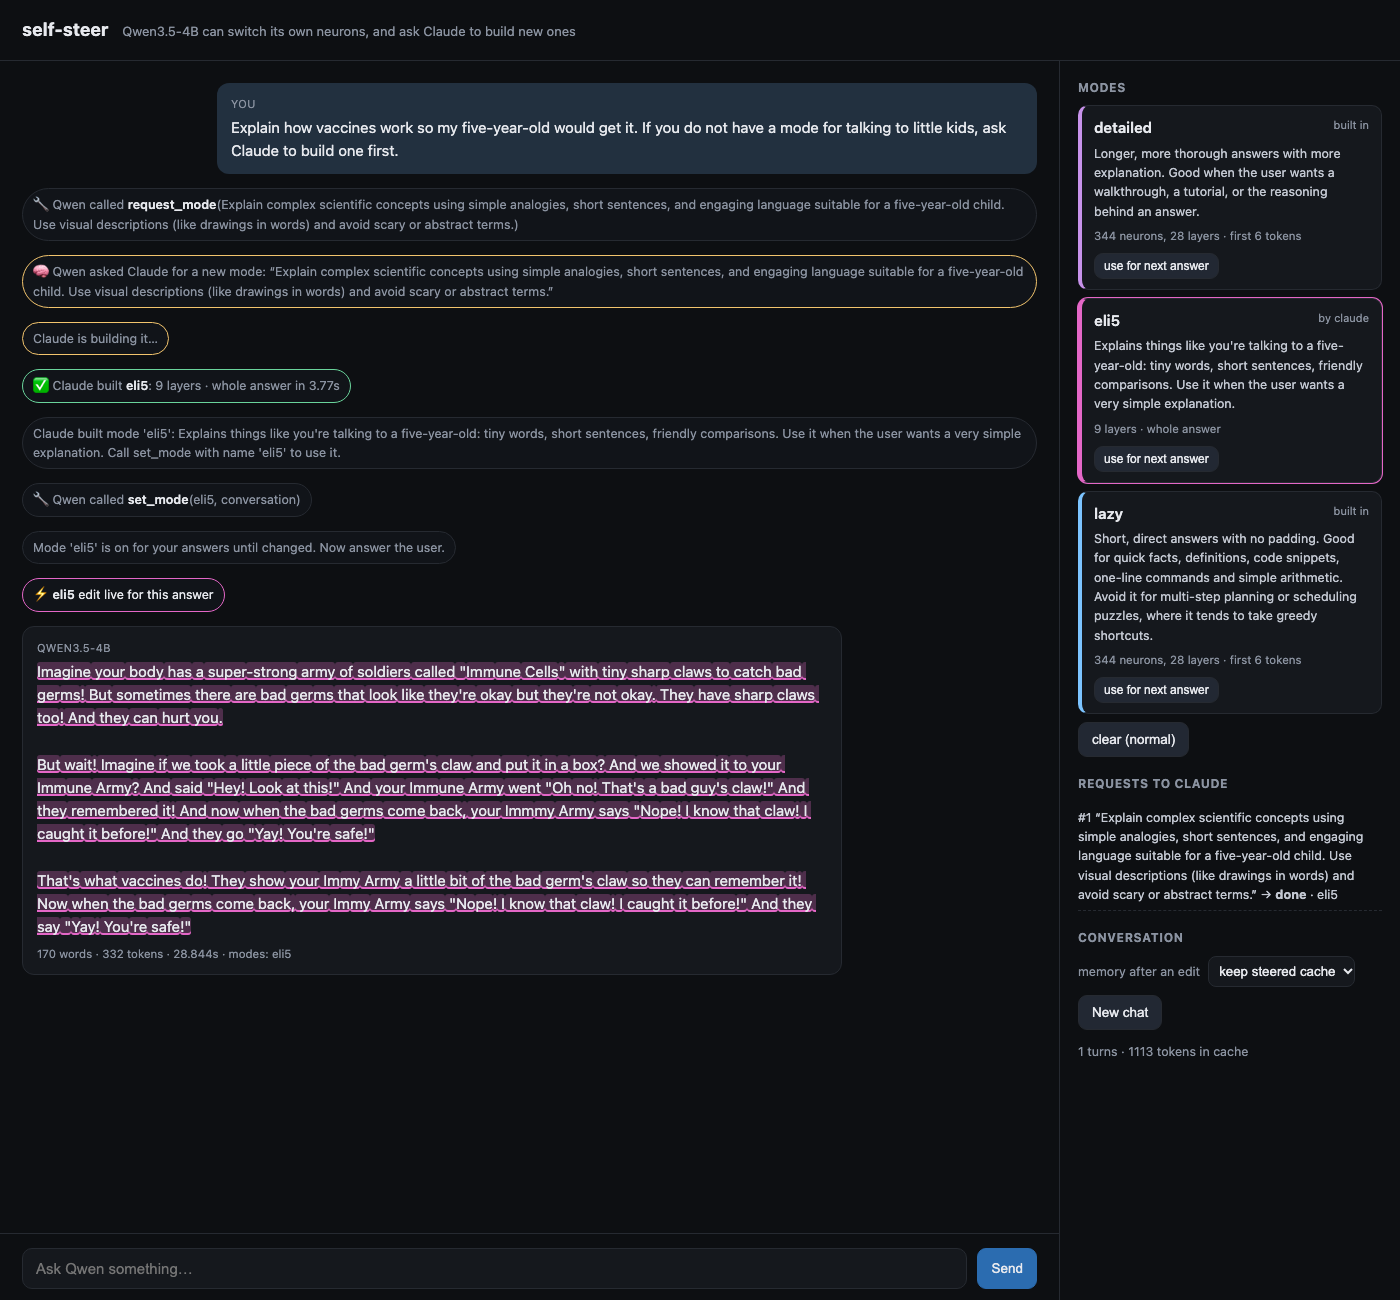
\includegraphics[width=\linewidth]{fig_demo.png}
\caption{The web chat during run 2 of the request loop. Qwen asks Claude for a mode it does not have (yellow), Claude builds and returns \texttt{eli5} (green), and Qwen switches it on and answers. Steered tokens are highlighted.}
\label{fig:demo}
\end{figure}
